
In this chapter, we study a driven multiqubit gate on the Krawtchouk chain. This system maps to free fermions, allowing us to obtain the complete energy spectrum, and allowing us to efficiently calculate the effect of driving fields in the fermionic picture. This particular system turns out to have an elegant interpretation of the eigengates in terms of the \textbf{so}(3) algebra, linking the eigengates to rotations on the sphere.  As a downside, the free-fermionic nature makes the actual resonantly driven gate scale unfavorably with larger numbers of qubits. 

\section{Analysing the model}
We assume a Hamiltonian, acting on $N=n+1$ qubits,
\begin{align}
H = &\sum_{x = 0}^{n-1} \frac{J_{x}(t)}{2} \big( X_{x}  X_{x+1} + Y_{x}  Y_{x+1} \big)  \nonumber \\
&+ \sum_{x=0}^n (\alpha_{x}(t) X_x + \beta_{x}(t) Y_x + \gamma_{x}(t) Z_x) ,
\label{eq:xyham}
\end{align}
where $\{ J_x, \alpha_x, \beta_x, \gamma_x \}$ are real, time-dependent functions over which we assume arbitrary and independent control. Note that in this specific case, we start counting the qubits at $x=0$. The specific choice of couplings
\begin{align}
J^K_x = -\frac{J}{2}  \sqrt{ (x+1)(n-x) }
\label{eqn:kccouplings}
\end{align}
gives rise to the so-called Krawtchouk chain Hamiltonian 
\begin{align}
H^K = \sum_{x = 0}^{n-1} {J^K_x \over 2} \big( X_{x}  X_{x+1} + Y_{x}  Y_{x+1} \big) .
\end{align}
We already noted some of the remarkable properties of this system in \cref{sec:transfer_single_exc}. The authors of Refs. \cite{Christandl2004,Nikolopoulos2004} observed that applying $H^K$ for a time $t = \pi/J$ exactly mirrors the left- and the right sides of the chain, allowing perfect state transfer (PST) between the ends of the chain. Another surprising application is that a $t = \pi/J$ pulse, acting on the product state $ |+\rangle^{\otimes N}$, gives the so-called {\it graph state} on a complete graph, which can be turned into a $N$-body GHZ state by 1-qubit rotations (see for example \cite{Clark2005}). For $N$ odd, $N=\pm1 \!\!  \mod \! 4$,
\begin{align}
& |{\rm GHZ}\rangle = \left( \frac{  |0^N \rangle  + |1^N \rangle  }{\sqrt{2}} \right) \nonumber \\
& \quad = e^{\pm i {\pi \over 4} } \exp[-i {\pi \over 4} X]^{\otimes N} \exp [-i {\pi \over J} H^K] |+\rangle^{\otimes N}.
\end{align}
The {\it Krawtchouk eigengates}\ $U_K$ we present below employ a `half-pulse' of duration $t=\pi/(2J)$, (\cref{eq:eigengate}), or rather a pulse combining the Hamiltonian $H^K$ with its dual $H^Z$, (\cref{eq:eigengatebis}). The half-pulse was previously used in Ref. \cite{Alkurtass2014} to generate the specific state $U_K \ket{1010 \ldots10}$, which turns out to be a rainbow state.

\paragraph{}
The Krawtchouk chain \cref{eq:xyham} is an example of an XX model spin chain, and we can use the techniques discussed in \cref{sec:XXmodel}. In particular, if $\alpha_x = \beta_x = 0$ for all $x$, then $H$ conserves the total spin in the $Z$-direction, hence the eigenstates have a well-defined total spin. We may interpret the spin-up excitations as fermionic particles through a Jordan-Wigner (JW) transform \cite{Jordan1928}:
\begin{align}
f^\dagger_x = [ \prod_{j < x} Z_{j} ] \sigma_x^-, \ \ f_x = [ \prod_{j < x} Z_{j} ] \sigma_x^+,
\label{eq:kcjw}
\end{align}
with $\sigma^+_x=(X_x + i Y_x)/2$,  $\sigma^-_x=(X_x - i Y_x)/2$.
Indeed, the operators $f_x$, $f_{x'}^\dagger$ obey canonical {\em anti-commutation} relations. The quadratic terms in \cref{eq:xyham} turn into
\begin{align}
H = \sum_{x=0}^{n-1} J_x(t) \left( f^\dagger_x f_{x+1} + \text{h.c.} \right)
\end{align}
and we conclude that the fermions are non-interacting.

\sloppy{Following Ref. \cite{Christandl2004}, we observe that action of $H^K$ on the Fock space states $\ket{0\dots 010 \dots 0}$ with Hamming weight 1 is} the same as the action of the angular momentum operator $L_X$ acting on the spin states of a particle with spin $s={n \over 2}$. Denoting the 1-particle state with the `1' at position $x$ as $\ket{ \{x \}}$, and the spin state with $L_z=m$ as $\ket{m}\rangle$, the identification is
\begin{align}
\ket{\{ x\}} \leftrightarrow \ket{m=x-{n \over 2}}\rangle.
\label{eq:id}
\end{align}
As a consequence, the eigenvalues $\lambda_k$ of 1-particle eigenstates $\ket{\{k \}}_{H^K}$ of $H^K$ make up a linear spectrum 
\begin{align}
\lambda_k = J(k - \frac{n}{2}), \quad k \in \{ 0, \dots, n \}.
\label{eq:spectrum}
\end{align}
The eigenstates $\ket{ \{k \}}_{H^K}$ can be expressed as \cite{Albanese2004}
\begin{align}
\ket{ \{ k \}}_{H^K} = \sum_{x=0}^n \phi^{(n)}_{k,x} \ket{\{ x\}}, \quad
\phi^{(n)}_{k,x} = \sqrt{ \frac{ {{n} \choose {x}}   }{  {{n} \choose {k}} 2^n } } K^{(n)}_{k,x},
\label{eqn:eigenstates}
\end{align}
where $K^{(n)}_{k,x}$ denote Krawtchouk polynomials,
\begin{align}
K^{(n)}_{k,x} = \sum_{j=0}^k (-1)^j {{x}\choose{j}} {{n-x}\choose{k-j}}.
\end{align}
The many-body eigenstates with $q$ particles are created by products of $q$ fermionic modes $c^\dagger_k=\sum_{x=0}^n \phi^{(n)}_{k,x} f^\dagger_x$,
\begin{align}
\ket{ \{ k_1 k_2 \dots k_q \}}_{H^K} = c^\dagger_{k_1} c^\dagger_{k_2} \ldots c^\dagger_{k_q}\ket{0}.
\end{align}
They satisfy
\begin{align}
H^K \ket{ \{ k_1 \dots k_q \}}_{H^K} = \left( \sum_{j=1}^q \lambda_{k_j} \right) \ket{\{ k_1 \dots k_q \}}_{H^K}.
\end{align}
Recall that the subscripts of kets denote the eigenbasis in which they are stated, which is well-defined thanks to the JW transformation. As all eigenvalues are (half-)integer multiples of $J$, all dynamical phases reset after time $t = 2 \pi M / J$ for $M$ (even) integer.  


\section{Mapping between eigenbases}
We now turn to a construction of an {\it eigengate}: a quantum circuit that efficiently generates the many-body eigenstates from states in the computational basis. We find two simple circuits that do the job,
\begin{align}
U_K & = \exp \left(- i {\pi \over 2J} H^Z \right)  \exp \left( - i {\pi \over 2J} H^K \right)  \exp \left( - i {\pi \over 2J} H^Z \right)
\label{eq:eigengate} \\
        & = \exp \left(  -i {\pi \over J}\frac{(H^K + H^Z) }{\sqrt{2}} \right).
\label{eq:eigengatebis}
\end{align}
Here $H^Z$ is the operator \cite{Kay2005}
\begin{align}
H^Z = {J \over 2} \sum_{x=0}^n (x-{n \over 2}) (\mathds{1}- Z)_x \ .
\end{align}
Its 1-body spectrum is the same, \cref{eq:spectrum}, as that of $H^K$, but the eigenvectors are very different: while $H^Z$ is diagonal on states $\ket{ \{ x_1 x_2  \ldots x_q \} }$ in the computational basis, $H^K$ is diagonal on the Krawtchouk eigenstates $\ket{ \{ k_1 k_2 \ldots k_q \} }_{H^K}$.

The key property is that the operator $U_K$ exchanges the eigenstates of $H^Z$ and $H^K$ and thus performs the change of basis that we are after. Labeling both sets $\{x_1 x_2 \ldots x_q\}$ and $\{k_1 k_2 \ldots k_q\}$ by a binary index $s$ taking values in $\{0,1\}^{n+1}$, we have 
\begin{align}
U_K \ket{s} = i^{q n} \ket{s}_{H^K} \hspace{4mm} \forall s \in \{0,1\}^{n+1},
\label{eqn:eigengate_summarized}
\end{align}
 or, in a different notation, 
\begin{align}
H^K U_K =  U_K H^Z .
\label{eq:intertwine}
\end{align}  
In fact, in this special case there is a third Hamiltonian,
\begin{align}
H^Y = \sum_{x = 0}^{n-1} {J^K_x \over 2} \big( Y_{x}  X_{x+1} -  X_{x}  Y_{x+1} \big)
\end{align}
which satisfies the \textbf{so}(3) commutation relations with $H^K$ and $H^Z$:
\begin{align}
[ H^{i} , H^{j} ] = i \epsilon_{ijk} H^k, \quad  i, j, k  \in \{ K, Y, Z \},
\end{align}
where $\epsilon_{ijk}$ is the totally antisymmetric tensor. The commutation relations allow us to picture the unitary $U_K$ as a rotation on the Bloch sphere, which agrees perfectly with the Hadamard transformation for $n=1$, $s=10$, $01$, up to a factor $i$.

 

\section{Resonant driving on Krawtchouk eigenstates}

\begin{figure}
  \begin{center}
    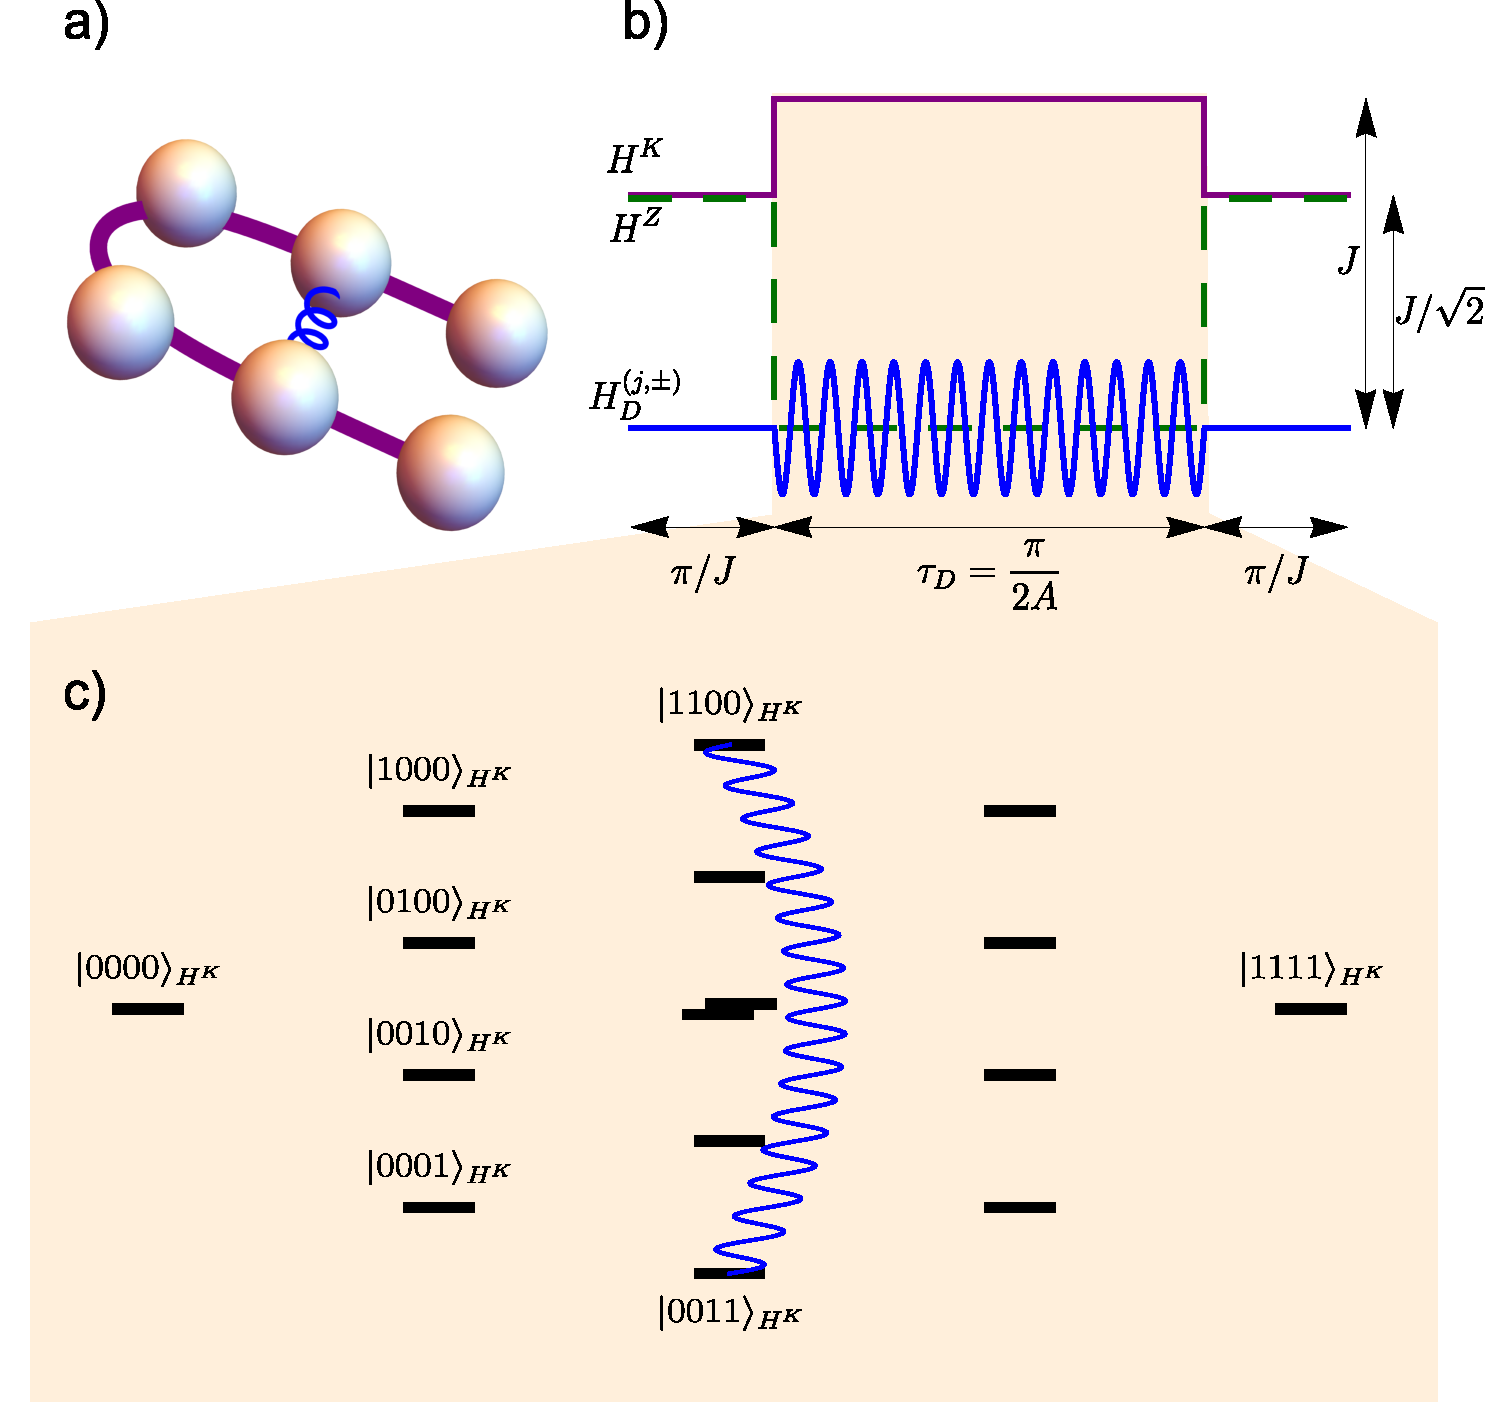
\includegraphics[width=.8 \textwidth]{krawtchoukN6_overview.pdf}
  \end{center}
  \caption{Overview of the proposed protocol for $\texttt{iSWAP}_N$ gates. a) The $N=6$ qubit chain (spheres) evolving under the Krawtchouk Hamiltonian (solid lines). The driving Hamiltonian $H_D^{(1,-)}$ is depicted as the corkscrew line. b) Field strengths as function of time. c) The spectrum of $H^K$ for $N=4$, with the resonant transition depicted as the curvy line.}
\label{fig:krawtchoukdriving}
\end{figure}



We first assume $N$ odd and consider a driving term coupling $\ket{0^{{n \over 2}+1} 1^{n \over 2}}_{H^K}$ and $\ket{1^{{n \over 2}+1} 0^{n \over 2}}_{H^K}$. The Hamming distance between these two states is $N$. Nevertheless it turns out that the two states can be coupled by a 1-qubit driving term. To see this, we write the JW transform as
\begin{align}
\sigma_x^- = [ \prod_{j < x} (1-2 \hat{n}_{j}) ] f^\dagger_x, \quad  \sigma_x^+ = [\prod_{j < x} (1-2\hat{n}_{j})]f_x
\label{eq:jw}
\end{align}
with $\hat{n}_j = f^\dagger_j f_j$. Targeting the middle qubit, $x={n \over 2}$, we observe that  the operator $\sigma_x^+$ contains precisely the right number of annihilation and creation operators operators to connect the two states. However, we find that amplitude of the matrix element is exceedingly small,
\begin{align}
{}_{H^K} \bra{1^{{n \over 2}+1} 0^{n \over 2}}   \sigma^-_{n \over 2} \ket{0^{{n \over 2}+1} 1^{n \over 2}}_{H^K} = (-2)^{-{n^2 \over 4}}.
\end{align}
Due to this, a resonant driving protocol based on this transition is problematic for $N \geq 5$.

The numbers work out better for a 2-qubit term driving a transition from $\ket{0^{
N \over 2} 1^{N \over 2}}_{H^K}$ to $\ket{1^{N \over 2} 0^{N \over 2}}_{H^K}$ for $N$ even. We propose the driving terms 
\begin{align}
& H^{(j,+)}_D = J_D \cos(\omega t) [\sigma_j^+ \sigma^-_{j+{N \over 2}} + \sigma_j^- \sigma^+_{j+{N \over 2}}],
\nonumber \\
& H^{(j,-)}_D = i J_D \cos(\omega t)  [\sigma_j^+ \sigma^-_{j+{N \over 2}} -  \sigma_j^- \sigma^+_{j+{N \over 2}}].
\end{align}
Note that the locations of the 1-qubit terms are precisely such that, together with the JW string, the required $\frac{N}{2}$ fermion creation \'{a}nd annihilation operators are contained in the driving fields. Making the string any longer would result in effectively less fermionic operators due to symmetry with respect to a global $\prod_x Z_x$ reflection. For $N=6$, we use the `central' 2-qubit driving operator that connects sites $x=1$ and $x=4$, which gives a coupling
\begin{align}
A = \frac{1}{2} | {}_{H^K} \bra{1^3 0^3}  H^{(1,-)}_D(t=0)  \ket{0^3 1^3}_{H^K} | = {5 \over 64} J_D
\label{eq:A}
\end{align}
whereas the largest matrix element of this operator in the 3-particle sector is ${9 \over 32} J_D$. Surprisingly, the matrix elements can be calculated explicitly even for larger $N$, as we show in \cref{sec:mtx_elts}. 

\cref{fig:krawtchoukdriving} depicts the protocol for the resonant driving. Having performed a first Krawtchouk eigengate, taking time $t_\text{eg} =\pi/J$, we turn on the combination
\begin{align}
H^K+H_D^{(1,-)}(t), 
\end{align}
starting at $t=0$, with the driving frequency $\omega=9J$ adjusted to the energy difference between $\ket{0^3 1^3}_{H^K}$ and $\ket{1^3 0^3}_{H^K}$. 
Choosing a driving time $t_d = 2\pi M/J$ with $M$ integer guarantees that all relative dynamical phases return to unity at time $t_d$. Choosing in addition $A={5 \over 64} J_D ={ \pi \over 2 t_d}={ J \over 4M }$ leads to a time-evolution that effectuates the transition
\begin{align}
\ket{0^31^3}_{H^K} \rightarrow i \ket{1^30^3}_{H^K}, \ \
\ket{1^30^3}_{H^K} \rightarrow i \ket{0^31^3}_{H^K}.
\end{align}
The protocol is completed by a second Krawtchouk eigengate of time $t_\text{eg}=\pi/J$. Summarizing,
\begin{align}
&  \ket{0^3 1^3} \stackrel{U_K}{\longrightarrow} \ket{0^3 1^3}_{H^K} \stackrel{U_D}{\longrightarrow} i \ket{1^3 0^3}_{H^K} \stackrel{U^\dagger_K}{\longrightarrow} i \ket{1^3 0^3}, 
\nonumber \\
&  \ket{1^3 0^3} \stackrel{U_K}{\longrightarrow} \ket{1^3 0^3}_{H^K} \stackrel{U_D}{\longrightarrow} i \ket{0^3 1^3}_{H^K} \stackrel{U^\dagger_K}{\longrightarrow} i \ket{0^3 1^3}.
\end{align}
A realistic implementation could apply an envelope over all control signals to guarantee smooth evolution of the fields. 

The same reasoning holds for systems of any (even) size $N$, leading to the operation $\texttt{iSWAP}_{t_1, t_2}$ that we presented earlier in \cref{eqn:udrive}, with $\phi = \pi$. In this case, we always have $t_1 = \ket{0^\frac{N}{2} 1^\frac{N}{2}}$ and $t_2 = \ket{1^\frac{N}{2} 0^\frac{N}{2}}$ (or vice versa). To avoid notational clutter, we refer to this operation as $\texttt{iSWAP}_N$ in the remainder of this chapter.


The procedure can be extended with the halfway inversion discussed in \cref{sec:halfwayinversion}. After driving for time $t_d/2$, we turn off $H^K$ and turn on $H^Z$ for time  $\pi/J$, which is equivalent to applying a gate of the form $\text{diag}(1,\pm i)$ on each qubit. This effectively performs perfect state transfer on the energy spectrum, mapping indices $k \rightarrow n-k$, or equivalently, a $\pi$-rotation around the $H^Z$-axis of the \textbf{so}(3) Bloch sphere. We complete the driving part of the protocol by driving once more for time $t_d/2$ followed by another $H^Z$-pulse of time $\pi/J$. This works without modification if $J t_d$ is an integer multiple of $\pi$, and for general $t_d$ when the phase $\phi$ of the driving function is adjusted in the second driving step. The halfway inversion is included in the numerics belows.


\section{Numerical results} 
\cref{fig:N4N6fidelities} plots the gate error, defined as in \cref{eq:gatefidelity}, for runtimes up to $M=20$.
%
\begin{figure}
  \begin{center}
    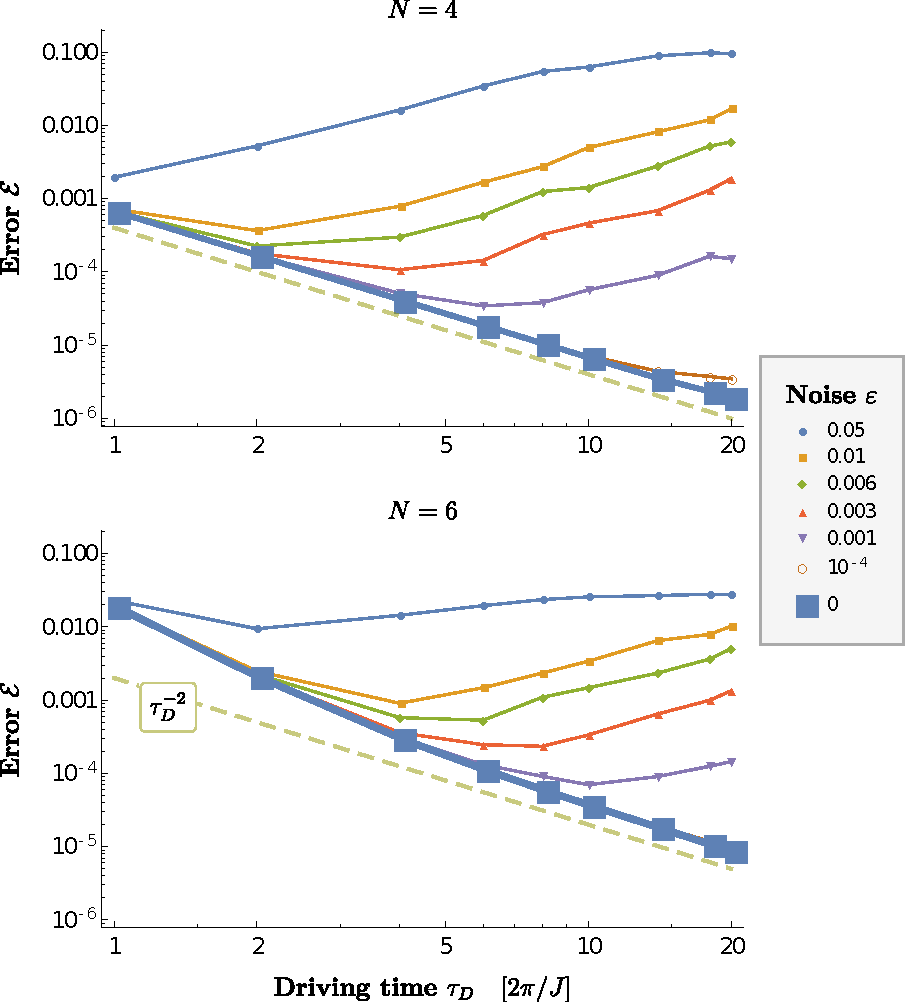
\includegraphics[width=.73 \textwidth]{drive_fids_n4_n6.pdf}
  \end{center}
  \caption{Fidelities of the resonant driving part of the $\texttt{iSWAP}_4$ and $\texttt{iSWAP}_6$ protocols, including the halfway inversion. The thick lines indicate the errors in the ideal case, thin lines under various values of noise $\varepsilon$. The errors fall off like $t_d^{-2}$ (dashed), until the noise $\varepsilon$ becomes the leading source of errors.}
\label{fig:N4N6fidelities}
\end{figure} 
%
The $N=4$ results have been obtained with driving operator 
\begin{align}
H^{(0,+)}_D(t) + H^{(1,+)}_D(t)
\end{align}
with resonant frequency $\omega=4J$. To probe the effect of non-ideal couplings $J_x^K$, we performed the same simulations under multiplicative noise, such that $J_x^K \rightarrow (1+ \varepsilon_x) J_x^K$ where $\varepsilon_x$ is chosen uniformly from $[-\varepsilon, \varepsilon]$. The multiplicative noise is independent of the actual field strengths $J$, making it largely independent of implementation details. The results shown are the averages of at least 180 simulations. 

From \cref{fig:N4N6fidelities}, we can read off the time taken by $\texttt{iSWAP}_N$ gates and make a comparison with the time taken by a fully entangling two-qubit gate. As comparison, we consider the gate formed by applying the similar $XX+YY$-type Hamiltonian on 2 qubits, leading to the operation $\texttt{iSWAP}_2$ \cite{Schuch2003}. The spatially varying Krawtchouk couplings, \cref{eqn:kccouplings}, grow up to strength $\max_x J^K_x = - \frac{J}{2} \frac{N}{2}$ (for $N$ even), and for a fair comparison we assume the couplings $J^K_x$ may grow no larger than $J^\text{max}/2$ for any $N$. Therefore, we penalize time as a function of $N$ by multiplying by a factor $\frac{N}{2} \frac{J}{J^\text{max}}$. The 2-qubit $\texttt{iSWAP}_2$ gate with coupling maximized at $J^\text{max}/2$ then takes time $\frac{\pi}{J^\text{max}}$. Note that on top of the driving time, the protocol requires 2 eigengates taking unpenalized time $t_\text{eg} = {\pi \over J}$, as well as a halfway inversion consisting of single-qubit gates of the form diag(1,$\pm i$), whose duration we neglect here. We also neglect the error due to a noisy eigengate, which turn out to be an order of magnitude lower than the driving errors encountered here \cite{Groenland2018}. 

For $N=6$, at sufficiently low noise $\varepsilon < 0.01$, we see an error $\mathcal{E}$ in the order of $10^{-3}$ for $M=4$ meaning it can be achieved in time $t =2 t_\text{eg} + t_d =10 \pi/J$. Penalizing for the largest couplings being 3 times larger than in the $N=2$ case, we conclude that our $\texttt{iSWAP}_6$ gate takes time equivalent to 30 2-qubit $\texttt{iSWAP}_2$ gates. For $N=4$ an error of well below $10^{-3}$ is already achieved with $M=1$ and we penalize with a factor 2, giving a runtime equivalent of 8 $\texttt{iSWAP}_2$ gates. Note that this is faster than the 10 gates required for a 3-qubit \texttt{Toffoli} as proposed in \cite{Schuch2003}. 



\section{Experimental implementations}
To our best knowledge, the only reported experiment in which non-trivial Krawtchouk couplings have been realized on spin-like qubits, is by Li et al. \cite{Li2018}. They use superconducting qubits with tunable couplings to mimic $H^K$ on four qubits, showing a transfer fidelity of 99.2\% in the subspace of a single spin excitation. It may be expected that simulating $H^K$ in sectors with more excitations will be less accurate, because the transmon-type qubits used in the experiment are technically nonlinear oscillators with bosonic excitations, which are prone to excitations outside of the computation subspace (going from state $\ket{0}$ or $\ket{1}$ into state  $\ket{2}$).

Other experiments, such as Refs. \cite{Perez-Leija2013,Chapman2016}, report to be the first to engineer Krawtchouk couplings and test PST, but use photonic waveguides which behave different when more than 1 particle is involved. Using NMR, experimental PST was demonstrated on 3 qubits using constant couplings \cite{Zhang2005}, and on up to 6 using iterative procedures \cite{Alvarez2010,Nikolopoulos2014}. 

For other platforms, various theoretical proposals for approximations of Krawtchouk spin chains can be found in literature. The NMR platform could implement spatially varying couplings by using techniques presented in Ref. \cite{Ajoy2013}, and numerical tests for this platform have been performed in, for example, Ref. \cite{Alkurtass2014}. Alternatively, cold atoms in a 1D optical lattice could be tuned to a regime where a two species Bose-Hubbard description reduces to an XX chain. The authors of Ref. \cite{Clark2005} present a numerical study exploring the viability of this scheme to realize graph state generation using Krawtchouk couplings. 




\section{Matrix elements of driving operators in free models}
\label{sec:mtx_elts}
In general, for driven multiqubit gates, it is essential to know the coupling strength between the two resonant states induced by the driving field. This calls for calculating quantities such as 
\begin{align*}
M = \bra{ t_1 } H_\text{drive} \ket{t_2}.
\end{align*}
For many-body eigenstates $t_1, t_2$, this can be a highly nontrivial problem, and in some cases one may have to resort to measurements on the hardware itself to find these values.


However, for models that can be mapped to free fermions, we may sometimes obtain exact expressions for the driving matrix elements. As in the case of the Krawtchouk chain, we consider driving fields that are functions of raising and lowering operators $\sigma^-$ or $\sigma^- \sigma^+$, acting between the states with the highest and lowest energy under some Hamiltonian $H$:
\begin{align} 
& M^{(1)}_j = _{H}\bra{ 1^{{n\over 2}+1} \ 0^{n \over 2} \ } \sigma_j^- \ket{\ 0^{ {n\over 2}+1} \  1^{n\over 2}}_{H} && (N \text{ odd}), \label{eq:mtx_elts_odd}
\\[2mm]
& M^{(2)}_{j,d} = _{H}\bra{1^{N\over 2} \ 0^{N\over 2} \ } \sigma_j^- \sigma_{j+d}^+ \ket{ \ 0^{N\over 2} \  1^{N\over 2}}_{H} && (N \text{ even}). 
\label{eq:mtx_elts_even}
\end{align}
Note that from these expressions, we can easily obtain the related values for the conjugate driving terms (see below). 


Now, let us apply the Jordan-Wigner transform as defined in \cref{eq:kcjw}, and assume that $H$ is diagonalized by the fermionic transformation 
\begin{align}
c^\dagger_k = \sum_{x=0}^n \phi^{(n)}_{k,x} f^\dagger_x,
\end{align}
where $\phi^{(n)}_{k,x}$ is a unitary matrix over indices $k,x$. These allow us to express \cref{eq:mtx_elts_odd,eq:mtx_elts_even} into  the values of $\phi^{(n)}_{k,x}$. 

\paragraph{Odd lengths} For the case of $N$ odd, we find that the only nonzero value of $M_j^{(1)}$ correspond to cases where $\sigma_j^-$ can be written in the form of $\frac{n}{2}$ annihilation operators, and $\frac{n}{2}+1$ creation operators (note that in our definition of the JW transformation, $\sigma^-$ corresponds to a fermionic creation operator). The only site $j$ on which the JW string is sufficiently long to produce this number of fermionic operators, is right in the middle, at site $j = \frac{n}{2}$. One might naively think that choosing $j$ larger than that would make the string longer, but by left-right mirror symmetry of the problem, one may reason that also for $j>\frac{n}{2}$ the value of $M^{(1)}_j$ is zero. 

For $j=\frac{n}{2}$, we may simplify the expression for $M_j^{(1)}$, through some rather tedious but otherwise straightforward algebra \cite{Groenland2018}. In the end, we obtain
%
\begin{align}
M^{(1)}_{j={n \over 2}} = 2^{n \over 2}  \begin{vmatrix} \phi^{(n)}_{ \{0,\ldots, {n \over 2} \} , \{ 0, \ldots, {n \over 2} \} } \end{vmatrix}  \begin{vmatrix}  \phi^{(n)}_{ \{0,\ldots,{n \over 2}-1\},\{{n \over 2}+1,\ldots,n\} } \end{vmatrix},
\label{eq:M1determinants}
\end{align}
%
where $\begin{vmatrix}  \phi_{\vec{x},\vec{y}} \end{vmatrix}$ denotes the minor of matrix $\phi$ with only rows $\vec{x}$ and columns $\vec{y}$ kept. 

Now, specializing to the case of the Krawtchouk chain, using
\begin{align*}
\begin{vmatrix} K^{(n)}_{ \{0,\ldots, {n \over 2} \} , \{ 0, \ldots, {n \over 2} \} } \end{vmatrix} &= (-2)^{n(n+2) \over 2} \\
\begin{vmatrix} K^{(n)}_{ \{0,\ldots,{n \over 2}-1\},\{{n \over 2}+1,\ldots,n\} } \end{vmatrix} &= (-2)^{n(n-2) \over 2}
\end{align*}
we find
\begin{align*}
M^{(1)}_{j={n \over 2}} = (-2)^{-n^2/4}.
\label{eq:mtx_elts_odd_scaling}
\end{align*}
The exponential decay of the matrix elements means that the driving times $t_d$ rise quickly as the number of qubits $n$ is increased, making the protocol unfeasible for large system sizes. 




\paragraph{Even lengths}
For the case of $M^{(2)}_{j,d}$, we similarly find that the JW string must fill precisely half of the chain, such that $d = \frac{n+1}{2}$ is the only non-zero case. We find
\begin{align*}
M^{(2)}_{j,d={n+1 \over 2}} = & \, 2^{n-1 \over 2} \begin{vmatrix} \phi^{(n)}_{ \{ j, \ldots, j+{n-1 \over 2}\} ,\{0,\ldots,{n-1 \over 2}\} } \end{vmatrix}  \begin{vmatrix}  \phi^{(n)}_{ \{j+1,\ldots,j+{n+1 \over 2} \},\{ {n+1 \over 2},\ldots, n\}} \end{vmatrix},
\end{align*}
which, together with
\begin{align*}
\begin{vmatrix}   K^{(n)}_{ \{ j, \ldots ,j+d-1\} , \{0, \ldots, \frac{n-1}{2} \} } \end{vmatrix} &= (-2)^{(n-1)(n+1) \over 8}, \\
\begin{vmatrix}  K^{(n)}_{ \{ j+1, \ldots,j+d\} , \{\frac{n+1}{2}, \ldots, n \} } \end{vmatrix} &= (-1)^{{(j+1)(n+1) \over 2}}(-2)^{(n-1)(n+1) \over 8} ,
\end{align*}
leads to closed-form expressions for the matrix elements $M^{(2)}_{j,d={n+1 \over 2}}$. For $n=5$ one finds $M^{(2)}_{j=1,d=3}=5/64$ while for $n=3$ we have $M^{(2)}_{0,2}=M^{(2)}_{1,2}=\sqrt{3}/8$.

Similar to the odd case, the values of $M^{(2)}$ fall off rapidly with $n$. For example, for $N=2,6,\ldots$, putting $j={n-1 \over 4}$, we find asymptotic behavior
\begin{align*}
M^{(2)}_{j={n-1 \over 2},d={n+1 \over 2}} \sim c_0 \,  c_1^n \, c_2^{n^2} n^{-1/6}
\end{align*}
with $c_2=2^{3/4}3^{-9/16}= 0.9065\ldots$. This implies that the run-time of the resonant driving protocol (in its current form) increases rapidly with $n$.




\paragraph{Conjugate terms} Lastly, we note that matrix elements of the conjugates of the discussed driving fields may have a different phase. In particular, for $N$ even, we find 
\begin{align*}
_{H^K}\bra{1^{N\over 2} \ 0^{N\over 2}  \ } \sigma_j^+ \sigma_{j+{N \over 2}}^- \ket{ \ 0^{N\over 2} \ 1^{N\over 2}}_{H^K}  = (-1)^{N\over 2} M^{(2)}_{j,{N \over 2}}.
\end{align*}
Hence, to achieve constructive interference, the optimal driving terms are of the form $H_D^{(j,+)}$ if $N/2$ is even, or $H_D^{(j,-)}$ if $N/2$ is odd. 




\subsection{Optimal scaling of matrix elements} 

One might wonder whether there exist systems for which the matrix elements in \cref{eq:mtx_elts_odd,eq:mtx_elts_even} do \emph{not} decrease as rapidly. In fact, it turns out that there exist transformations $\phi^{(n)}_{k,x}$ such that $M^{(1)}_{j={n \over 2}}$ is \emph{constant} in $n$. We can derive this as follows, focusing specifically on the case of $N$ \emph{odd}. Hadamard's inequality states that the determinant of a matrix $\phi$ is bounded by the product of the sizes of it's rows:
%
\begin{align*}
| \det(\phi) | \leq \prod_{i=0}^n |\phi_i|.
\end{align*}
%
Here, $\phi_i$ denotes the vector obtained by taking the $i$th row (or column) of $\phi$, and $|\phi_i|$ is the normal vector length (2-norm). For \cref{eq:M1determinants}, we obtain 
%
\begin{align*}
|M^{(1)}_{j={n \over 2}}| \leq 2^{n \over 2} \left[  \prod_{x=0}^{\frac{n}{2} - 1}   | \phi_{x,\{0, \ldots, \frac{n}{2} \} } | | \phi_{x,\{\frac{n}{2} + 1, \ldots, n \} } |  \right] | \phi_{ \frac{n}{2},\{0, \ldots, \frac{n}{2} \} } |.
\end{align*}
%
On the other hand, by unitarity, for each value of $x$ we require that 
%
\begin{align*}
| \phi_{x,\{0, \ldots, \frac{n}{2} \} } |^2 + | \phi_{x,\{\frac{n}{2} + 1, \ldots, n \} } |^2 = 1
\end{align*}
%
The matrix element is optimized when $| \phi_{x,\{0, \ldots, \frac{n}{2} \} } | = | \phi_{x,\{\frac{n}{2} + 1, \ldots, n \} } | = \frac{1}{\sqrt{2}}$ for all $x$, except for the case $x=\frac{n}{2}$ where $|\phi_{ \frac{n}{2},\{0, \ldots, \frac{n}{2} \} } | = 1$. This intuitively means that the matrix $\phi_{k,n}$ has, on it's first $\frac{n}{2}$ \emph{columns}, equal amplitude on the $\frac{n}{2}$ uppermost and $\frac{n}{2}$ lowermost \emph{rows}. This gives the bound
\begin{align}
|M^{(1)}_{j={n \over 2}}| \leq 1.
\end{align}
This bound is actually \emph{tight}, because  Hadamard's inequality is satisfied whenever the relevant blocks consist only of orthogonal sets of vectors. These blocks are, in our conventions, precisely the upper-left and bottom-left quarters of the matrix $\phi^{(n)}_{k,x}$. In such cases, the matrix element $|M^{(1)}_{j={n \over 2}}|= 1$ indicates that the two states $\ket{ 1^{{n\over 2}+1} \ 0^{n \over 2} \ }_H$ and $\ket{\ 0^{ {n\over 2}+1} \  1^{n\over 2}}_{H}$ are almost identical: they differ from each other only by a bitflip $X$ on the middle qubit (and possibly an irrelevant phase). 

An explicit example of a unitary matrix that satisfies our bound, is
\begin{align*}
\phi' = 
\begin{pmatrix}
            1/\sqrt{2} & 0 & 0 & 0 & -1/\sqrt{2} \\               
            0 & 1/\sqrt{2} & 0 & -1\sqrt{2} & 0 \\               
            0 & 0 & 1 & 0 & 0  \\
            0 & 1/\sqrt{2} & 0 & 1\sqrt{2} & 0 \\               
            1/\sqrt{2} & 0 & 0 & 0 & 1/\sqrt{2}         
\end{pmatrix}.
\end{align*}
This $N=5$ case trivially generalizes to larger sizes. In the fermionic picture, the state $\ket{\ 0^{ {n\over 2}+1} \  1^{n\over 2}}_{H}$ looks like $\frac{n}{2}$ particles, each of which is in a superposition between two sites $x$ and $n-x$. The other state, $\ket{ 1^{{n\over 2}+1} \ 0^{n \over 2} \ }_H$, looks similar, but with an additional particle localized at site $x=\frac{n}{2}$. In the spin language, these correspond precisely to the \emph{rainbow states} we discussed before in \cref{sec:transport-half-filling}. In fact, \emph{every left-right-symmetric XX chain} has these rainbow states as eigenstates, hence for each of these systems, the corresponding fermionic diagonalization transformation $\phi^{(n)}_{k,x}$ has a certain ordering in which $|M_j^{(1)}| = 1$. This ordering is precisely such that the states which are \emph{symmetric} under mirroring the chain left-to-right (i.e. $x \rightarrow n-x$) occupy the bottom-most rows of $\phi^{(n)}_{k,x}$, and the \emph{anti-symmetric} states are in the top-most rows (or the other way around). 

Given that our prefered driving operator has such a large matrix element between these rainbow states, one might wonder if we can use these for a resonantly driven gate. The good news is that an eigengate is readily available: because the rainbow states are eigenstates of \emph{any} left-right symmetric XX-chain, we may use the Krawtchouk eigengates $U_K$ to create rainbow states from simple computational basis states. This specific eigengate was already observed in Ref. \cite{Alkurtass2014}, in the context of a quench that creates maximal entanglement between the left and right halves of the chain. 

The bad news is that it is hard to create a unique energy gap between the rainbow states. On left-right symmetric chains, the states with even and odd parity are alternating in the spectrum. Therefore, the rainbow states are of the form $U_K \ket{0101 \ldots }$ and $U_K \ket{1010 \ldots }$, and their energies are close to $0$. The sector with roughly half filling contains an exponentially large number of states (in $N$), and these are most dense around the energy $0$. Due to the spectral crowding, we find that near-resonant states become increasingly problematic in driven protocols as $N$ increases. 

The rainbow states can be pushed towards the bottom or top of the spectrum by using couplings that decay exponentially towards the ends to the chain, as is the case for the rainbow Hamiltonian discussed in Ref. \cite{Ramirez2018}. In the limit of increasingly strong decay of the couplings, a rainbow state becomes the ground state of the system, but unfortunately we find that this ground state is strongly degenerate, prohibiting the unique transition we hope to find. 

\section{Conclusion}
In conclusion, for the XX spin model, it is possible to find reasonably realistic eigengates and unique transitions. We study a specific example on the Krawtchouk chain. Unfortunately, we find that the matrix elements decay rapidly with $N$, making large multiqubit gates unfeasible. On the other hand, large matrix elements that are constant in $N$ can be found, but we argue that these correspond to frequency-crowded parts of the spectrum. 

An interesting direction of future research would be to find a best-of-both-worlds combination, where perhaps the matrix elements decay slowly, but are such that a sufficiently unique transition exists. 



